
\opchapter{پایگاه داده}\label{chap3}

\section{تعریف}\label{sec1:chap3}

پایگاه دادهٔ
\lr{MySQL}\footnote{MySQL:‌ \TNR/mai.es·kyoo·el/}
 یک سیستم مدیریت پایگاه داده رابطه‌ای (\lr{RDBMS}) است که برای ذخیره، مدیریت و دسترسی به داده‌ها استفاده می‌شود. \lr{MySQL} یکی از پایگاه‌های داده محبوب و قدرتمند است که توسط شرکت \lr{Oracle} توسعه داده شده است. این پایگاه داده از زبان ساختار یافته پرس و جو (\lr{SQL}) برای تعامل با داده‌ها استفاده می‌کند.

\lr{MySQL} امکانات گوناگونی را برای مدیریت پایگاه داده فراهم می‌کند، از جمله:

\begin{itemize}[nosep]
	\def\labelenumi{\arabic{enumi}.}

	\item
	ایجاد و مدیریت جداول.
	\item
	جستجو و استخراج داده‌ها.
	\item
	نظارت بر امنیت.
	\item
	پشتیبانی از تراکنش‌ها.
	\item
	پشتیبانی از اتصال همزمان.
	\item
	پشتیبانی از رویکردهای بالا.
\end{itemize}

با این تعریف پایگاه دادهٔ \lr{MySQL} را می‌توان یک سیستم مدیریت پایگاه داده
رابطه‌ای محبوب و قدرتمند دسته بندی کرد که از زبان \lr{SQL} برای مدیریت داده‌ها
استفاده می‌کند و امکانات زیادی را برای طراحی، مدیریت و استفاده از پایگاه
داده‌ها فراهم می‌کند.

در اینجا از \lr{MySQL} در سمت \lr{server} استفاده شده و اطلاعات کاربران، توکن‌های
دسترسی، فراداده‌های کاربران، دستورات ارسال شده توسط دستگاه‌های سمت کاربر و
همچنین لیست وضعیت‌های رخ داده و در حال رخ دادن در خودرو ذخیره شده‌اند.


\paragraph{توابع تحلیل فضایی}\label{par1:sec1:chap3}

\lr{MySQL} دارای قابلیت ذخیرهٔ \lr{polygon}های جغرافیایی است که اجازه می‌دهد تا
نقاط و شکل‌های هندسی چندضلعی را در جداول دیتابیس ذخیره کند و عملیات
محاسبات مکانی را روی آن‌ها انجام دهد.

اضافه بر موارد گفته شده، یکی از قابلیت‌های مفید \lr{MySQL} وجود توابع تحلیل
فضایی
\LTRfootnote{Spatial Analysis Functions.}
 است. که امکان ذخیره‌سازی محدوده‌های
جغرافیایی مشخص‌شده توسط کاربر محیا می‌کند، و همچنین امکان اجرای یک \lr{query}
برای بررسی وجود یک نقطه درون آن محدوده، که در اینجا برای تشخیص وجود
خودرو در محدودهٔ مشخص شده توسط کاربر استفاده شده‌است.

در مجموع ویژگی‌های موجود عبارت‌اند از:

\begin{itemize}[nosep]
	\item
	نوع داده: در \lr{MySQL}، \lr{polygon}های جغرافیایی به صورت اشیاء جغرافیایی ذخیره
	می‌شوند. این شئ می‌تواند یک چندضلعی بسته، یک لایه منطقی یا یک نقشه در
	نظر گرفته شود.
	\item
	ذخیرهٔ داده: پلتفرم \lr{GIS} از جداول داده‌های جغرافیایی به عنوان کشویی برای
	ذخیرهٔ اشیاء جغرافیایی استفاده می‌کند. به همین دلیل، می‌توانید
	\lr{polygon}های جغرافیایی را به صورت \lr{filed} در جداول خود ذخیره کنید.
	\item
	عملیات مکانی: یکی از ویژگی‌های قوی \lr{MySQL} امکان انجام عملیات مکانی روی
	داده‌های جغرافیایی است. با استفاده از توابع مکانی مانند \lr{ST\_Contains}،
	\lr{ST\_Intersects} و \lr{ST\_Distance}، می‌توانید عملیات پرس‌وجوی پیچیده را روی
	\lr{polygon}هایی که در جداول ذخیره شده‌اند، انجام دهید.
	\item
	هندسه مکانی:
	\lr{MySQL}
	 قادر به ارائهٔ ویژگی‌های هندسی مانند محاسبهٔ مساحت و
	محدودهٔ \lr{polygon}های جغرافیایی است. توابعی مانند \lr{ST\_Area}، \lr{ST\_Length} و
	\lr{ST\_Perimeter} این امکان را فراهم می‌کنند.
\end{itemize}

بنابراین، به کمک قابلیت ذخیرهٔ \lr{polygon}های جغرافیایی در \lr{MySQL} می‌توانید
منطق مکانی و پرس‌وجوی پیچیدهٔ وابسته به مکان را در سیستم‌های خود پیاده‌سازی
کنید.


\subsection{جداول پایگاه‌داده}\label{sub1:sec1:chap3}

لیست جداول تعریف شده در سمت \lr{server} به صورت ذیل است.

از طرفی به دلیل افزایش کارایی اجرا و سرعت بیشتر و همچنین سبکی سعی شده
جداول حدالامکان ساده طراحی و مشخص شده‌باشند و اطلاعات به راحتی قابل
پرس‌وجو توسط \lr{MySQL} باشند.

همچنین برای ذخیرهٔ نشست‌های کاربران از برنامه‌های موجود همانند
\lr{Telegram}\footnote{
	تلگرام یک برنامهٔ شبکهٔ اجتماعی و یک پیام‌رسان است.
}
ایده گرفته شده و قابلیت تمایز و اتصال چند نشست از طرف یک کاربر ممکن است،
و همچنین اطلاعات کاربران مشابه به ذخیرهٔ اطلاعات به صورت عمومی‌تر و امکان
تغییر راحت‌تر به صورت یک جدول از کلید و داده
(\lr{key/value}) ذخیره شده‌اند،‌این
عمل از ذخیرهٔ‌ داده‌ها در
\lr{WordPress}\footnote{
	وردپرس یک
	\lr{CMS}
	محبوب برای ساخت وبسایت‌ها است.
}
ایده‌برداری شده.

\subsection{لیست جداول و توضیحات مربوط}\label{sub2:sec1:chap3}

\begin{itemize}[nosep]
	\item
	نوع دستگاه (\lr{device\_type}) در این جدول نوع دستگاه‌های ممکن لیست شده،‌که
	به صورت پیش‌فرض شامل \lr{vehicle}، \lr{android}، \lr{linux}، \lr{win}، \lr{ios} است.

	\textbf{ویژگی‌ها}: شناسه (\lr{id}), نام (\lr{name}), توضیحات (\lr{desc})
	\item
	حالت (\lr{states})

	حالت‌های موجود برای هر دستور، محدوده یا کاربر، که به صورت پیش‌فرض شامل
	مقادیر \lr{activated}، \lr{disabled}، \lr{suspended}، \lr{readonly} است.

	\textbf{ویژگی‌ها}: شناسه (\lr{id}), نام (\lr{name}), توضیحات (\lr{desc})
	\item
	نوع وضعیت و دستورات (\lr{fields})

	این جدول شامل نوع وضعیت‌ها و دستورات موجود در جدول‌های \lr{statuses} و
	\lr{commands} است.

	داده‌های در این دو جدول به صورت \lr{JSON} برای راحتی تلفیق و همچنین راحتی
	تعریف انواع دادهٔ جدید در صورت نیاز تعریف شده، که به واسطهٔ این جدول
	امکان دسته‌بندی راحت‌تر داده‌ها در جدول \lr{commands} را ممکن می‌سازد.

	\textbf{ویژگی‌ها}: شناسه (\lr{id}), نام (\lr{name}), توضیحات (\lr{desc})
	\item
	کاربران (\lr{users})

	جدول کاربران شامل شناسهٔ کاربر، توکن (\lr{token}) دسترسی و همچنین آخرین
	زمان دسترسی کاربر است.

	\textbf{ویژگی‌ها}: شناسه (\lr{id}), وضعیت (\lr{stid}), توکن (\lr{token}), زمان (\lr{utc})
	\item
	نشست‌های کاربران (\lr{users\_sessions})

	برای ایجاد دستورات و ارسال داده به سرور هر کاربر با توجه به هر دستگاه
	نیازمند ایجاد یک نشست برای دستگاه موجود است، بدین حالت بعد از ایجاد
	نشست کاربر از توکن احراز هویت خود برای ورود به سیستم استفاده کند.

	همچنین در این جدول برخی از ویژگی‌های مهم‌تر دستگاه مقصد نیز نگه‌داری
	می‌شوند.

	\textbf{ویژگی‌ها}: شناسه (\lr{id}), کاربر (\lr{uid}), نوع دستگاه(\lr{tid}), وضعیت
	(\lr{stid}), توکن احراز هویت (\lr{authtoken}), شناسهٔ یکتای دستگاه (\lr{mac}), زمان
	ایجاد (\lr{register}), زمان آخرین دسترسی (\lr{access}), آدرس \lr{IP} دستگاه (\lr{ip}),
	(\lr{port})
	\item
	محدوده‌های مشخص شده(\lr{boundaries})

	محدوده‌های مشخص شده به کاربر اجازهٔ ایجاد بخش‌ها و محدوده‌های جغرافیایی   را می‌دهد، که توانایی ایجاد رفتارهای متفاوت را به کاربر برای هر بخش را   بدهند.

	\textbf{ویژگی‌ها}: شناسه (\lr{id}), جلسه (\lr{sid}), وضعیت (\lr{stid}), محدودهٔ
	جغرافیایی (\lr{poly}), زمان (\lr{utc})
	\item
	آخرین وضعیت خودرو (\lr{latest\_status})

	آخرین وضعیت خودرو شامل یک مقدار \lr{JSON} است که شامل داده‌های تجمیع شده از آخرین وضعیت خودرو است، که برای دسترسی سریع‌تر و نیاز به بررسی تمامی  دستورات موجود را مهیا می‌کند.

	\textbf{ویژگی‌ها}: شناسه (\lr{id}), کاربر (\lr{uid}), مجموعهٔ آخرین تغییرات در یک
	جا به صورت \lr{JSON} (\lr{data}), زمان (\lr{utc})
	\item
	تمام وضعیت‌های گزارش شده (\lr{statuses})

	در این جدول وضعیت‌های گزارش‌ها توسط هر خودرو لیست شده‌اند.

	\textbf{ویژگی‌ها}: شناسه (\lr{id}), جلسه (\lr{sid}), نوع مقدار (\lr{fid}), محتوا به
	صورت \lr{JSON} (\lr{data}), زمان (\lr{utc}), وضعیت دسترسی و مشاهده (\lr{accessed})
	\item
	دستورات ارسال شده (\lr{commands})

	این جدول شامل دستورات ارسال شده توسط کاربر است، دستورات ارسال شده در   قالب \lr{JSON} هستند، برای مثال: نمونه‌ای از دادهٔ یک دستور برابر
	‍‍\lrm{\{"doors":{[}false,false,false,false{]}\}} است.

	\textbf{ویژگی‌ها}: شناسه (\lr{id}), جلسه (\lr{sid}), نوع مقدار (\lr{fid}), محتوا به
	صورت \lr{JSON} (\lr{data}), زمان (\lr{utc}), وضعیت دسترسی و مشاهده (\lr{accessed})
	\item
	فرادهده‌های مربوط به هر کاربر (\lrm{user\_meta})

	مشابه به هر سیستمی هر کاربر شامل فرا‌داده‌هایی مانند پست الکترونیکی، شمارهٔ همراه و
	\ldots{}
	 است که این جدول برای ذخیرهٔ این نوع از داده‌ها   قرار گرفته، که داده‌ها به صورت ترکیبی از کلید و داده در این جدول ذخیره   شده‌اند، که یک رابطهٔ یک به چند با جدول کاربر دارد.

	\textbf{ویژگی‌ها}:
	شناسه (\lr{id}), کاربر (\lr{uid}), نام فرا داده (\lr{key}), مقدار   فرا داده (\lr{value})
\end{itemize}

\section{دیاگرام}\label{sec2:chap3}
در ذیل دیاگرام مربوط به جداول پایگاه‌دادهٔ ایجاد شده در سمت سرور فراهم شده‌است.
که شامل ۸ جدول مرتبط به هم هستند.
\begin{figure}[!h]
	\centering
	\footnotesize
	\frame{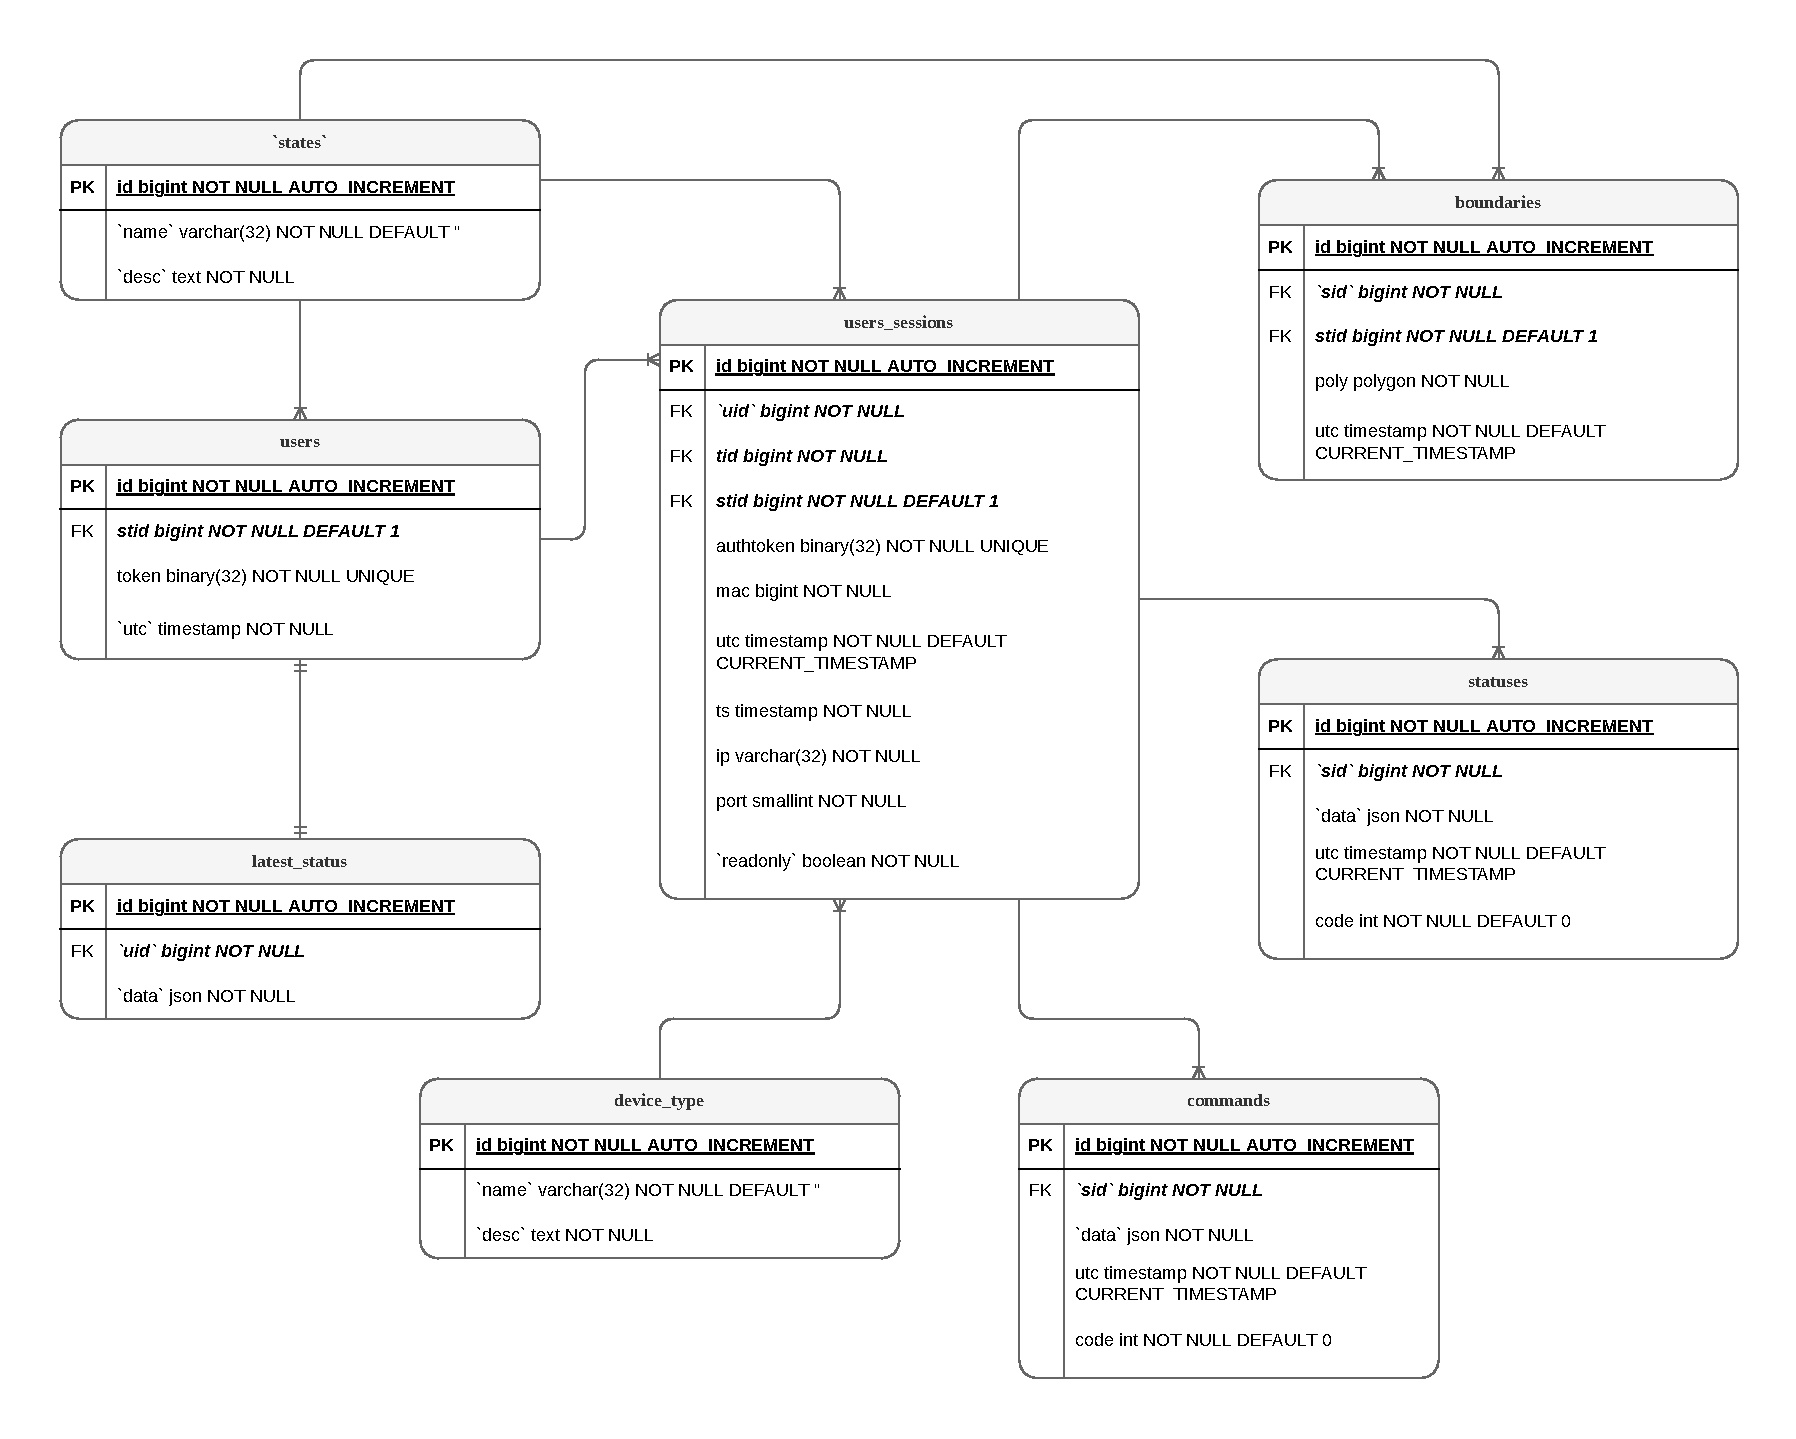
\includegraphics[width=\textwidth]{../diagrams/database.pdf}}
	\hspace*{1cm}
	\normalsize
	\label{fig2:sec3:chap3}
	\caption{دیاگرام مجتمع پایگاه داده}
\end{figure}


\section{روابط}\label{sec3:chap3}
دیاگرام موجود در بخش قبل نشان‌دهندهٔ روابط میان جدول‌های پایگاه‌داده است، که در مرکزیت این روابط و پایگاه‌داده، جدول
\emph{نشست‌های کاربر}
 قرار دارد که یک ارتباط
\textit{چند به یک}
  با جدول
\emph{کاربران}
 دارد.

همچنین جداول \emph{دستورات}، \emph{محدوده‌ها} و \emph{وضعیت‌ها} نیز ارتباط چند به یک با جدول نشست‌ها دارند، اما جدول آخرین وضعیت‌ها تنها یک ارتباط یک به یک با جدول کاربران دارد، بدین منظور که هر کاربر تنها توانایی برخورداری و کنترل یک خودرو است و برای هر خودرو نیز تنها یک ردیف از
\emph{آخرین وضعیت‌ها}
در پایگاه‌داده ذخیره می‌شود.

\section{رخداد‌ها}\label{sec4:chap3}
در \lr{MySQL}، رخدادها کدی هستند که به صورت خودکار اجرا می‌شوند و در پاسخ به رویدادهایی که در جداول دیتابیس رخ می‌دهند، عملیات خاصی را انجام می‌دهند.

در واقع، رخدادها از قوانین مجموعه قراردادهای \lr{SQL} بهره می‌برند و با یک سری دستورات \lr{SQL}، به عنوان یک واکنش به عملیاتی که روی داده‌ها انجام می‌شود، اجرا می‌شوند که به دلیل احتمالی حجم زیاد \textit{دستورات} و \textit{وضعیت‌های خودرو} رویدادی نیز برای برای پاک کردن داده‌ها در دامنهٔ زمانی مشخص شده قرار داده‌شده.

در حال حاضر در رویداد مشخص شده داده‌های قدیمی در بازه‌های روزانه از جداول پایگاه‌داده پاک‌سازی می‌شوند.

\begin{latin}
	\small
	\begin{lstlisting}[language=sql,caption={automated remove vehicle's status event}]
		CREATE EVENT vehicle_status_cleaner
		ON SCHEDULE AT CURRENT_TIMESTAMP + INTERVAL 1 DAY
		ON COMPLETION PRESERVE
		DO DELETE LOW_PRIORITY FROM db_cardian.statuses WHERE utc < DATE_SUB(NOW(), INTERVAL 1 DAY)
	\end{lstlisting}
\end{latin}